\documentclass[10pt]{article}
\usepackage[paperwidth=33.1in,paperheight=23.4in,margin=0.7in]{geometry}  % A0 landscape-ish, poster ratio
\usepackage{graphicx}
\usepackage{booktabs}
\usepackage{amsmath,amssymb}
\usepackage{xcolor}
\usepackage{multicol}
\usepackage{enumitem}
\usepackage{titlesec}
\usepackage{helvet}
\renewcommand{\familydefault}{\sfdefault}

\setlist{nosep,leftmargin=1.1em}
\setlength{\columnsep}{0.55in}
\setlength{\columnseprule}{1pt}
\renewcommand{\columnseprulecolor}{\color{blue!40}}

\definecolor{accent}{RGB}{31,63,126}
\definecolor{accent2}{RGB}{186,28,28}
\definecolor{blockbg}{RGB}{238,244,252}

% Section headers as poster blocks
\titleformat{\section}
  {\Large\bfseries\color{white}}
  {}{0pt}{}
  [{\vspace{-6pt}\color{accent}\rule{\linewidth}{3pt}}]
\titlespacing{\section}{0pt}{10pt}{6pt}

\newcommand{\blockhead}[1]{%
  \par\vspace{8pt}\noindent
  \colorbox{accent}{\parbox{\dimexpr\linewidth-12pt\relax}{%
    \vspace{4pt}\hspace{6pt}{\Large\bfseries\color{white}#1}\\[4pt]}}%
  \par\vspace{6pt}}

\begin{document}
% ================= TITLE BANNER =================
\begin{center}
\colorbox{accent}{\parbox{0.97\textwidth}{%
  \centering\vspace{14pt}
  {\Huge\bfseries\color{white}
   CW305-Based Physical Security Evaluation of ASCON-128:\\[6pt]
   Deep-Learning Side-Channel Analysis and\\[4pt]
   Clock-Glitch Fault Injection}\\[12pt]
  {\large\color{white!90!black}
   Prajwal R \quad$\bullet$\quad Prajwal G S Basavaraj \quad$\bullet$\quad
   Sachin S \quad$\bullet$\quad Nitesh}\\[4pt]
  {\normalsize\color{white!90!black}
   Dept.\ of Electronics and Communication Engineering, PES University, Bengaluru, India}\\[4pt]
  {\normalsize\color{white!90!black}\textit{VLSID 2027 Student Research Forum}}\vspace{12pt}
}}
\end{center}
\vspace{10pt}

\begin{multicols}{3}

% ============================================================
\blockhead{Motivation \& Platform}
ASCON-128, the NIST SP~800-232 lightweight AEAD standard, is entering
constrained FPGA deployments, yet hardware-measured leakage and fault
data on the \emph{official unmasked NIST LWC core} remain sparse. We
ask: what does a real Artix-7 implementation leak under power analysis
and clock glitching --- and which apparent results are measurement
artifacts?

\centering
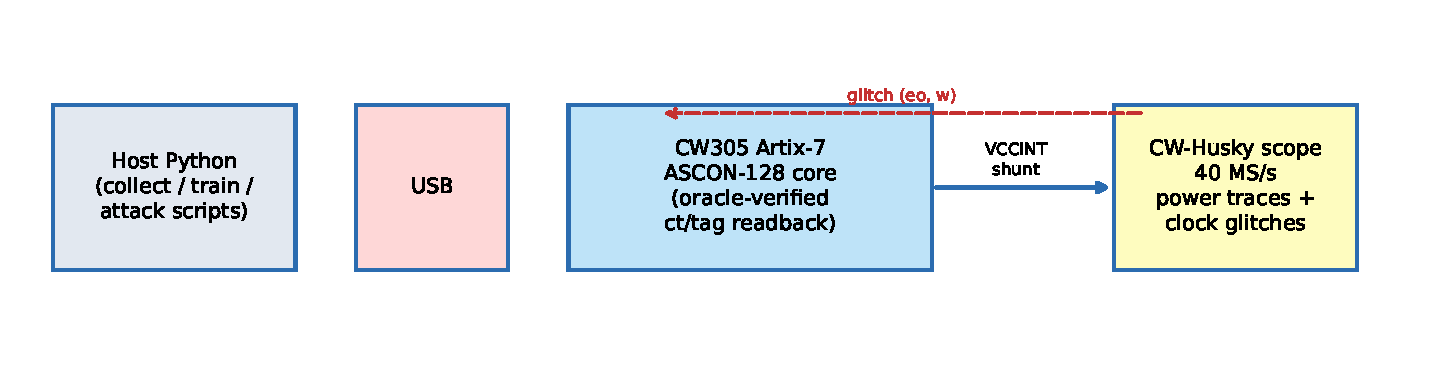
\includegraphics[width=0.96\linewidth]{figs/platform_diagram.pdf}\par
\vspace{4pt}
\begin{itemize}
\item CW305 Artix-7 + CW-Husky scope; \textbf{40\,MS/s against
  10\,MHz crypto clock} (4 samples/cycle), VCCINT shunt, per-query
  trigger on \texttt{tio4}.
\item \textbf{Byte-exact oracle verification:} every stored trace is
  accepted only after its ct/tag readback matches a software reference
  (5/5 NIST KATs on the bitstream).
\item Random keys for profiling; nonce-repetition averaging $M$ as an
  explicit SNR knob ($\sqrt{M}$ gain); fixed AD/PT blocks.
\end{itemize}

% ============================================================
\blockhead{Deep-Learning SCA: the S-box Target}
One CNN/MLP profile per S-box column (64 columns $\times$ 2 unknown key
bits $\Rightarrow$ 4 hypotheses/column), trained on 80/20 random-key
splits; HW labels 0--5; empty-class-weighted loss.

\centering
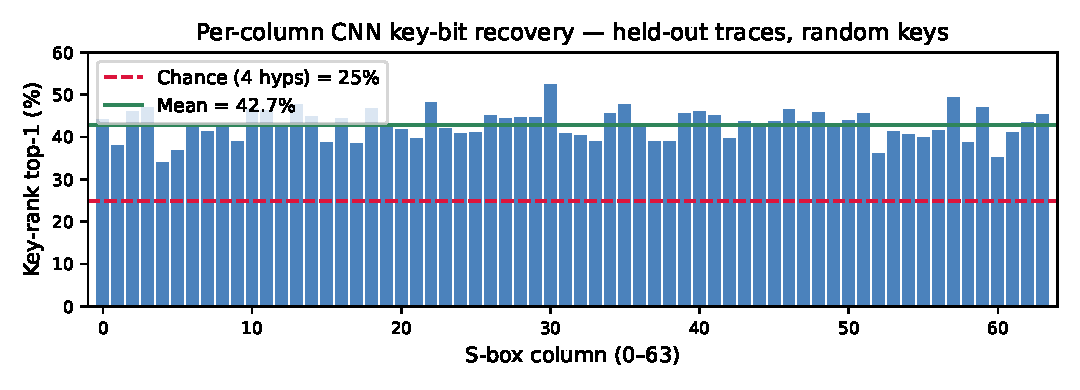
\includegraphics[width=0.98\linewidth]{figs/keyrank_columns.pdf}\par
\vspace{4pt}
\begin{itemize}
\item \textbf{Per-column key-bit recovery} on held-out random-key
  traces: key-rank top-1 \textbf{42.7\% mean vs 25\% chance}; all 64
  columns above chance, 0/64 below 30\% (offline-verified;
  HW-class top-1 28--35\% vs 16.7\% uniform chance).
\item \textbf{Profiling-domain gap} is real and column-specific:
  offline profiles transfer poorly to the live board across sessions.
\item \textbf{Live on-board fine-tuning} closes the gap: 300 board
  traces at a known key $\Rightarrow$ 90.7\% training accuracy vs 72\%
  majority floor; the fine-tuned column recovers correct bits on the
  live board at $M{=}1$, while unfine-tuned columns sit at chance.
\end{itemize}

\blockhead{Full-Key Assembly Strategy}
Divide-and-conquer: (1) closed-loop attack per column $\Rightarrow$
posterior $P(h_c\mid\mathbf{t})$ over 4 hypotheses; (2) top-1 per
column $\Rightarrow$ 128-bit candidate; (3) verify by re-encrypting a
fresh nonce against the oracle; (4) bounded enumeration over the
least-confident columns ($2^m$). Budget $\approx 64 \times q(M) \times
2^m$. \textbf{Characterized as ongoing work:} the empirical 64-column
run needs per-column on-board fine-tuning --- a measurement-budget
constraint, not an information-theoretic one.

\columnbreak

% ============================================================
\blockhead{The SNR Lever: Nonce-Repetition Averaging}
\centering
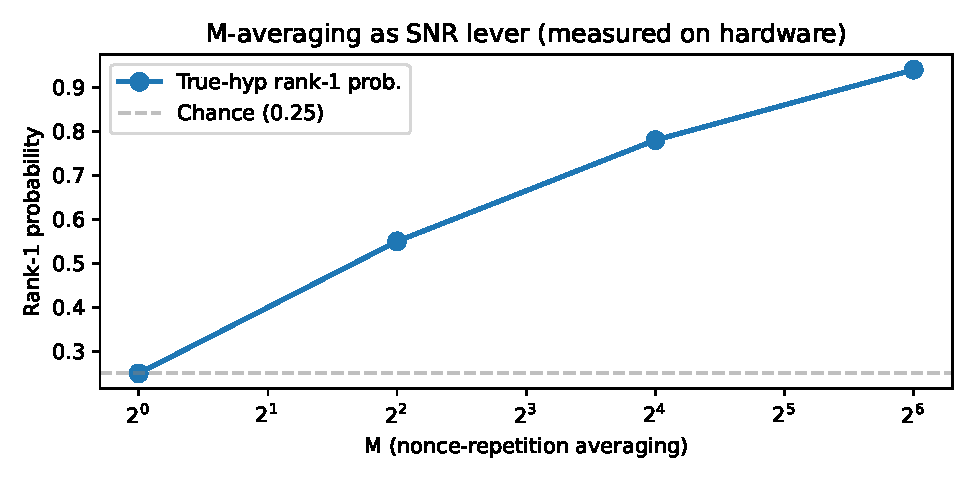
\includegraphics[width=0.62\linewidth]{figs/m_averaging.pdf}\par
\vspace{4pt}
\begin{itemize}
\item Repeating one separating nonce $M$ times and averaging raises
  per-query SNR by $\sqrt{M}$.
\item True-hypothesis rank-1: \textbf{0.25 at $M{=}1$ (chance)}
  $\rightarrow$ \textbf{0.94 at $M{=}64$} (on-board probe, one column).
\item In the closed loop, $M{=}64$ shortens convergence
  15 $\rightarrow$ 9 queries/column.
\item The align-then-z-score pipeline removes jitter and DC drift so
  the full $\sqrt{M}$ gain survives end-to-end.
\end{itemize}

\blockhead{Closed-Loop Adaptive Key Recovery}
Posterior-scoring chosen-nonce attack on one column, $M{=}1$:
converges to the \textbf{correct} hypothesis in \textbf{32 queries,
posterior 0.999}, using only public information (power + chosen
nonces). Per-column scope (2 of 128 bits) stated honestly; full-key
assembly is the divide-and-conquer step above.

\blockhead{Masked-Core Comparison (d=1, 2-share)}
Same pipeline against the threshold-implemented core (9{,}151 traces,
random keys): round-1 S-box at \textbf{chance for every architecture}
(CNN, MLP, centered-product MLP). First-order masking confirmed
effective on hardware; the unmasked-vs-masked contrast isolates
masking as the causal variable. Cost: $\approx 1.8\times$ throughput,
$\approx 2.1\times$ area (LUTs).

% ============================================================
\blockhead{Clock-Glitch Fault Injection}
\centering
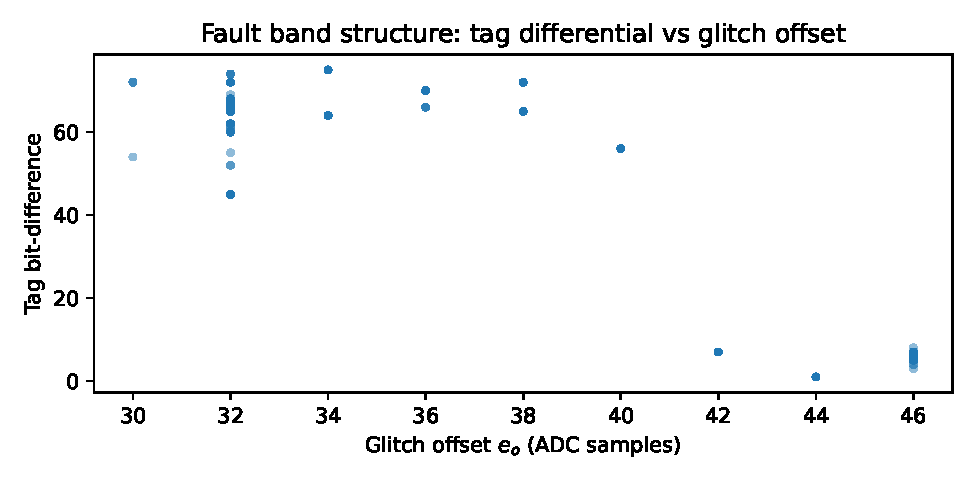
\includegraphics[width=0.78\linewidth]{figs/band_structure.pdf}\par
\vspace{2pt}
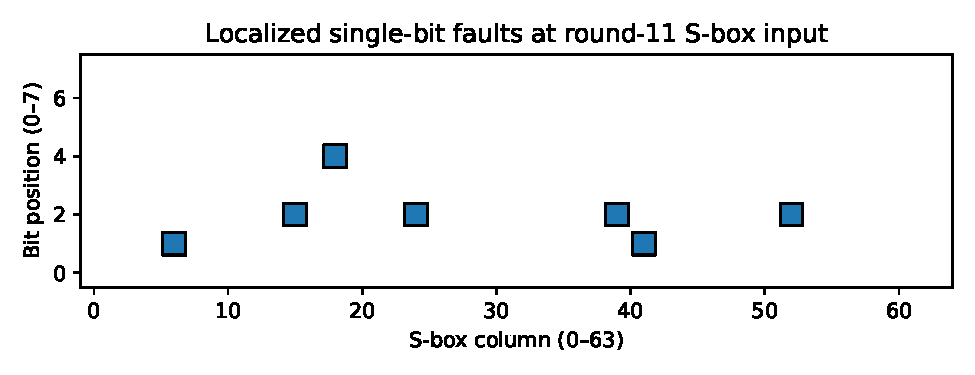
\includegraphics[width=0.62\linewidth]{figs/fault_map.pdf}\par
\vspace{4pt}
\begin{itemize}
\item Sweeping glitch offset $e_o\in[28,50]$ reveals a stable fault
  band at $e_o{=}41$: large tag differentials (27--41 bits), two
  landing positions (sub-offset 0 / 3359).
\item From 406 band hits over 153 distinct tags, \textbf{12 clean
  single-bit round-11 faults} localized to exact (column, bit) ---
  10 distinct state columns --- each verified by exact faulty-tag
  match under a simulated single-bit flip.
\item \textbf{Data-selected placement:} each nonce faults exactly one
  column, reproducibly; DFA coverage bounded at one column/query.
  Nonce-set engineering ($\approx$266 nonces, coupon-collector bound)
  or multi-glitch schedules restore full-column coverage.
\item Burst glitches fault 400/400 queries but as multi-bit
  superpositions (30+ bits), not composable single-bit faults or round
  skips.
\end{itemize}

\columnbreak

% ============================================================
\blockhead{Five Leakage-Validation Gates}
Confident false positives are the norm on this platform, not the
exception. Each trap ships with a reusable detection gate.

\begin{enumerate}
\item \textbf{Prior-driven edge scores.} A per-trace log-likelihood
  ``edge'' reported $+0.398$\,nats on data where every classifier sat
  at the majority floor --- the edge measured the prior.
  \emph{Gate:} held-out accuracy must beat the majority-class floor.
\item \textbf{Prior-only profiles + separating-nonce selection.}
  A below-floor profile outputs the prior regardless of trace; the
  picker then inverts it $\Rightarrow$ posterior 0.993 on the
  \emph{wrong} hypothesis (0\% label match).
  \emph{Gate:} profiles entering a closed loop must clear the floor
  gate.
\item \textbf{Public-nonce shortcut labels.} At a fixed key, column
  labels are a function of two \emph{public} nonce bits; a model
  reading nonce-load activity ``cracks'' vacuously.
  \emph{Gate:} profile on random keys; verify against re-encryption.
\item \textbf{Key-reload register-bus artifact.} A capture loop that
  rewrites the key before every trace embeds key-write bus activity:
  $|r|\approx0.6$ at the load samples, up to 64/64 columns of fake
  key-bit leakage.
  \emph{Gate:} the leak must survive a fixed-key capture (nonces
  varying).
\item \textbf{Structured-key / free-alignment false recovery.} A
  ramp-key template attack reported 75.8\% per-bit recovery; the
  reversed ramp scores identically and the bit-inverted key scores
  \emph{higher} (76.6\%) --- impossible for a genuine read (must invert
  to $\approx$24\%). Blind random-key capture: no signal.
  \emph{Gate:} inversion-invariance + structure-preserving nulls +
  blind random-key control.
\end{enumerate}

\blockhead{Attack-Surface Synthesis}
\begin{itemize}
\item \textbf{Unmasked + PA:} S-box target trainable (42.7\% key-rank
  top-1 vs 25\% chance); fine-tuning closes the domain gap;
  per-column closed-loop recovery at posterior 0.999 in 32 queries;
  $\sqrt{M}$ averaging is the SNR lever. Gap: 64-column assembly
  (measurement budget).
\item \textbf{Unmasked + FI:} verified single-bit round-11 faults with
  exact localization (12 cases, 10 columns); burst faults multi-bit;
  placement data-selected. Gap: intra-query column coverage.
\item \textbf{Masked core:} factorable target suppressed to chance
  (9{,}151 traces); masking performs at first order on hardware.
\item \textbf{Artifacts:} five trap classes with gates; the key-reload
  bus and structured-key/roll traps are, to our knowledge, unreported
  for LWC hardware evaluation.
\end{itemize}

\blockhead{Conclusions}
\begin{enumerate}
\item An oracle-verified CW305 platform delivers three
  hardware-verified result classes on the official unmasked NIST LWC
  ASCON-128 core.
\item DL-PA recovers per-column round-1 S-box key bits; per-column
  closed-loop recovery converges at posterior 0.999 in 32 queries; the
  $\sqrt{M}$ lever lifts rank-1 from 0.25 to 0.94.
\item Clock glitching yields verified single-bit round-11 faults at
  exact (column, bit) positions --- with data-selected placement as a
  documented DFA constraint.
\item Five reusable gates separate signal from artifact; two trap
  classes are platform-general and unreported to our knowledge.
\item First-order masking (d=1) is confirmed effective on the same
  platform.
\item Full 128-bit assembly is enabled and characterized as ongoing
  work.
\end{enumerate}

\blockhead{Acknowledgments}
PES University ECE (ISFCR); NewAE CW305/Husky platform. Poster
accompanies the VLSID 2027 Student Research Forum submission.

\end{multicols}
\end{document}
